\chapter{Introduction}
\label{ch:introduction}
\ref{pub:review} gives a detailed overview of many of the concepts and literature necessary to understand the experimentation and results described in later chapters - thus it makes up the bulk of this introductory chapter. In fact, sections discussing \acrfullpl{ztc} and \ce{H2} and \ce{CH4} storage are outside the scope of the practical parts of this work, but give some insight into the broader field of porous materials, adsorption, and small molecule capture/storage. Nonetheless there was some important detail which was not included in the publication, thus sections \ref{s:ccs} and \ref{s:adsorption_porosity} are included to discuss \ce{CO2} capture, and the general theories of adsorption and porosity, respectively.

\newpage
\section{\texorpdfstring{\ce{CO2} capture}{CO2 capture}}
\label{s:ccs}

Methods for \ce{CO2} capture as an add-on to industrial processes can be divided into three principal, broad groups; (i) oxy-fuel combustion, (ii) pre-combustion capture and (iii) post-combustion capture.\citep{kanniche2010pre} Oxy-fuel combustion is not a true \ce{CO2} capture method, but provides a means to more facile \ce{CO2} capture by producing a highly pure stream of \ce{CO2} meaning that gas separation is not necessary priory to capture.\citep{stanger2015oxyfuel, wall2009overview} Pre-combustion capture on the other hand involves the gasification of the fuel source using steam and oxygen, forming a mixture of \ce{H2} and \ce{CO} which is known as syngas. The \ce{H2} can be used as a fuel, while in a similar manner to oxy-fuel combustion, the \ce{CO} is converted to pure \ce{CO2} for ease of capture.\citep{jansen2015pre} Post-combustion capture does not require any of these complex treatments - \ce{CO2} is simply separated and captured from existing flue streams.\citep{wang2017review, samanta2012post} Thus, this method may be considered the the most versatile of the three.

As stated in \ref{pub:review}, \textbf{section 1} the principal commercial mode of post-combustion \ce{CO2} capture is \textit{via} chemical capture using liquid amines. This process is plagued by high costs due to the degradation of the amine solvent as well as corrosion of equipment.\citep{aronu2009solvent, dutcher2015amine, delgado2018degradation} Membrane-based \ce{CO2} capture and separation doesn't rely on chemical regeneration as the requisite membrane material simply selectively allows \ce{CO2} to travel through it while excluding other molecules due to their size.\citep{adewole2013current, ramasubramanian2011recent} The (theoretically) pure stream of \ce{CO2} is then captured at the other side. In order for this to work, high pressures must be use to force \ce{CO2} through the membrane; this can often lead to membrane degradation.\citep{powell2006polymeric} As a result of these problems, a third category of \ce{CO2} capture materials is under a lot of investigation - that is, solid porous sorbents which are not plagued by high regeneration costs or degradation. These include \acrshortpl{mof},\citep{Ding2019Carbon, qian2020mof} zeolites,\citep{Siriwardane2005Adsorption, Krishna2010silico} and of course porous carbons.\citep{Zhu2015Naturally, Chen2019Template, Xia2011Superior, Sevilla2016Highly} 

Candidates for solid \glspl{adsorbent} applied to \ce{CO2} capture are typically exploited for swing adsorption processes such as \acrfull{psa}, \acrfull{vsa} or \acrfull{tsa}. This type of process relies on \gls{adsorption} taking place at some pressure (\acrshort{psa}, \acrshort{vsa}) or temperature (\acrshort{tsa}) after which \ce{CO2} can be regenerated by changing the condition; typically this means reducing the pressure or increasing the temperature to facilitate desorption.\citep{bahamon2018energetic, hedin2013adsorbents, Zhao2018Synthesis, adewole2013current, ho2008reducing}  \acrshort{psa} and \acrshort{vsa} only differ in that the former captures \ce{CO2} at elevated pressure and regenerates by reducing to ambient pressure; whereas the latter performs capture at ambient pressure and release occurs at vaccuum. Thus \acrshort{vsa} is more cost effective, however both of these pressure-based solutions are more desirable than \acrshort{tsa} as they can be performed at the elevated temperatures present in flue gases.\citep{ho2008reducing, adewole2013current, Pirngruber2013} Due to the different physical conditions used to capture and regenerate \ce{CO2} in each of these adsorptive processes, selection of solid sorbent is based on porosity. For example, materials for \acrshort{psa} should have a high specific surface area and possess minimal microprosity while for \acrshort{vsa} pore size is more important than overall surface area (see \ref{pub:review}, \textbf{figure 3.}).\citep{ho2008reducing, Chou2004, Presser2011Effect} Physisorbents such as \acrshortpl{mof} and zeolites have also been recently applied to the newer field of \acrfull{dac}, which may prove a necessary, complementary technology to post-combustion capture.\citep{kumar2015direct, mcqueen2021review, deutz2021life} Selectivity for \ce{CO2} over \ce{N2} is particularly important in \acrshort{dac} due to \ce{CO2}'s low partial pressure in the air. The selectivity is usually facilitated \textit{via} moieties with high chemical affinity for \ce{CO2}, but nonetheless porosity is likely to play a role in the performance of these materials.\citep{kumar2015direct, darunte2016direct, deng2021comparative}

\section{Physisorption \& porosity}
\label{s:adsorption_porosity}
Porous materials possess an interconnected pore system where pores are defined as voids which are deeper than they are wide.\citep{mcnaught1997compendium, Thommes2015Physisorption} Additionally, pores are defined as being able to contain fluid, which indirectly gives a minimum width for voids to be considered pores of \qty{2.6}{\angstrom}, as this is the kinetic diameter of the smallest practical fluid specie, \ce{He}.\citep{Thommes2015Physisorption, Lide2007Handbook} The ability of porous materials to contain fluids has led to the use of the phenomenon of adsorption being used to characterise their porosity. That is, knowledge of the behaviour of the system when the material is enriched with a fluid is utilised to understand pore size, shape and interconnectivity. In particular, so-called \gls{physisorption} is exploited wherein \gls{adsorbate}-\gls{adsorbent} interactions do not include any sort of chemical attraction but instead rely on non-bonding forces\citep{Thommes2015Physisorption} - thus hypothetically, structure ought not be significantly conflated with surface chemistry. What follows is a discussion of the various types of pore structures and associated adsorption phenomena. More specifics on the derivations of porosity from \gls{physisorption} isotherms is available in \ref{pub:review}, \textbf{section 3.4.2.} as well as section \ref{ss:porosimetry}.


\subsection{Pore characteristics and filling mechanisms}
\label{ss:pore_filling}

\begin{figure}[hb!]
    \centering
    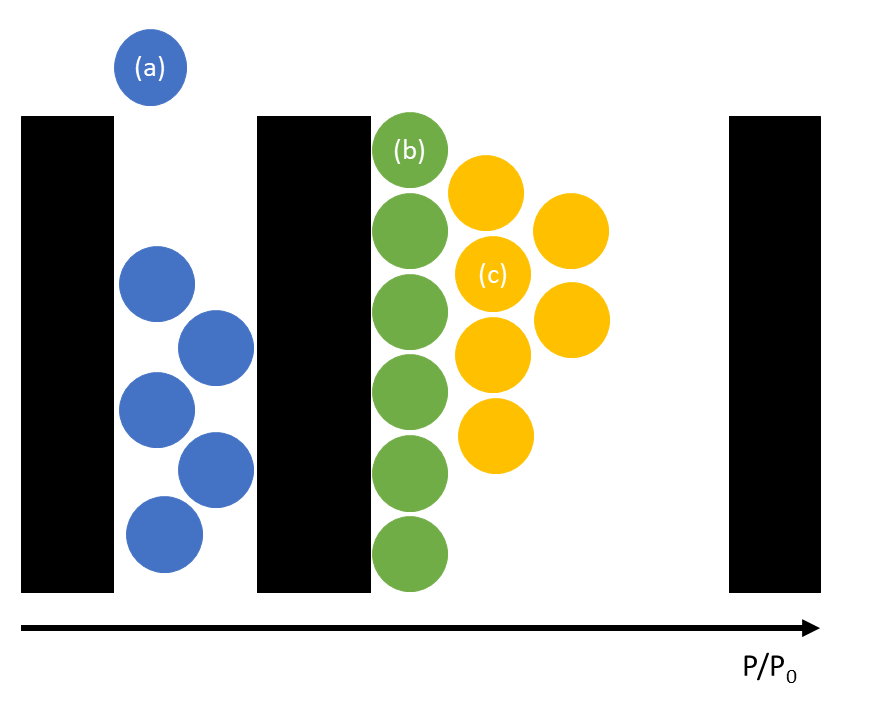
\includegraphics[width=\columnwidth, keepaspectratio]{1-introduction/figs/pore_filling.png}
    \caption{The three principle pore filling mechanisms, in order of their occurence with increasing relative pressure; (a) micropore filling; (b) completion of the monlayer in mesopores; and (c) multilayer adsorption.}
    \label{fig:filling}
\end{figure}

The \acrfull{iupac} defines ranges of pore sizes according to the mechanisms of pore filling by an \gls{adsorbate}.\citep{Thommes2015Physisorption} The three main mechanisms; \gls{micropore} filing; monolayer adsorption; and multilayer adsorption are illustrated in figure \ref{fig:filling}. Specifically, \glspl{micropore} (\qty{<20}{\angstrom})\citep{mcnaught1997compendium} are filled at ultralow relative pressures, and are characterised by strong heats of adsorption due to complementary \gls{adsorbate}-\gls{adsorbent} interactions from all pore walls.\citep{dubinin1989fundamentals} The subdivision into \glspl{ultramicropore} (\qty{<7}{\angstrom}) and \glspl{supermicropore} (\qtyrange[range-units=single]{7}{20}{\angstrom})\citep{mcnaught1997compendium} is derived from the fact that pores narrower than \qty{7}{\angstrom} can fit two adjacent rows of \ce{N2} molecules,\citep{Thommes2015Physisorption} and thus have the highest degree of pore wall potential overlap. \Glspl{mesopore} (\qtyrange[range-units=single]{20}{500}{\angstrom})\citep{mcnaught1997compendium} are characterised by being large enough to allow monolayer adsorption. That is, all adsorbed molecules are in contact with the surface and are not significantly influenced by attraction to an opposing pore wall.\citep{gregg1967adsorption, yang1997gas} As pressure increases, repulsive \gls{adsorbate}-\gls{adsorbate} interactions are overcome so that additional \gls{adsorbate} molecules adsorb on top of the monolayer - this process is known as multilayer adsorption. The widest pore size classification is \glspl{macropore} which are larger than 500 \unit{\angstrom}\citep{mcnaught1997compendium} and are not easily characterised by isothermal gas adsorption experiments, instead necessitating the use of mercury intrusion porosimetry for determination of porosity.\citep{abell1999mercury, gregg1967adsorption, haynes1973pore} In addition to these principal adsorption processes, in \glspl{mesopore} capillary condensation can occur at relative pressures greater than \num{\sim0.2} wherein the adsorbate enters a liquid-like state despite being below saturation pressure. This can lead to hysteresis in the resultant isotherm which is discussed in more depth in section \ref{ss:iso_interpretation}.\citep{Thommes2015Physisorption, monson2012understanding}

While few materials show uniform pore shape, idealised shape is defined by \acrshort{iupac} according to five characteristic shapes; cylindrical, slit, funnel, sphere, and ink-bottle.\citep{rouquerol1994recommendations, kaneko1994determination, zdravkov2007pore} For example while aluminium oxides typically have cylindrical pores,\citep{zdravkov2007pore} \glspl{turbostratic carbon} are usually assumed to have slit-shaped pores,\citep{Everett1976Adsorption, Jagiello20132D, Lastoskie1993} although carbide-derived carbons have been shown to possess cylindrical or spherical pores.\citep{kurig2016suitability} Zeolites have a broad range of pore shapes.\citep{park2002effect} 

In addition to shape and size, pores are also defined by their degree of accessibility. Figure \ref{fig:pore_accessibility} illustrates this type of pore classification. In general, pores can be termed as `closed' or `open', based on whether or not they have an accessible entrance. In the case of open pores, these are further subdivided into `through' pores wherein both ends of the pore are accessible, and `blind' pores wherein only one end of the pore is accessible. In addition, porosity can be formed through undulations on the surface, provided that the depth of these undulations is greater than the width. These are known as `external pores'. However open pores are not necessarily accessible to an adsorptive, that is there entrance may be smaller than the adsorptive molecule - these pores are termed as `chemically closed'. This can occur for ink-bottle pores with a narrow neck, or for very narrow slit or cylindrical pores.\citep{rouquerol1994recommendations, kaneko1994determination, zdravkov2007pore} Porosimetry is only able to quantify apparent porosity as defined by `true' open pores (i.e. not chemically closed) and indeed for gravimetric adsorption applications this is the the only kind of meaningful porosity. However, closed pores nonetheless contribute to a materials bulk density and thus can influence \textit{volumetric} uptake capacity for an adsorptive.

\begin{figure}[t!]
    \centering
    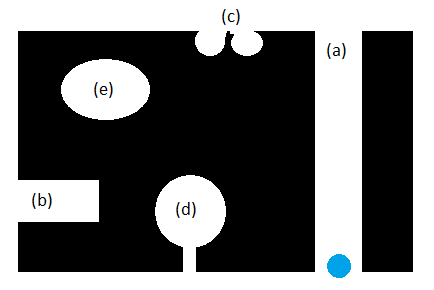
\includegraphics[width=\columnwidth, keepaspectratio]{1-introduction/figs/pore_accessibility.png}
    \caption{The diferent types of pores classified according to their accessibility; (a) an open, through pore; (b) an open, blind pore; (c) external pores; (d) a chemically closed pore; and (e) a closed pore. The small blue dot indicates the probe molecule size.}
    \label{fig:pore_accessibility}
\end{figure}

The final characteristic of porous structures is porosity hierarchy. Materials like \acrshortpl{mof} and zeolites typically possess uniform or unimodal porosity,\citep{WeitkampZeolites, Siriwardane2005Adsorption, Ding2019Carbon, lin2009hydrogen} whereas \glspl{turbostratic carbon} typically have multiple- or even a continuous range of (i.e. hierarchical) pore widths.\citep{Li2020Hierarchical, Sevilla2014Energy, Xia2008Hierarchical, Balahmar2017Biomass} The pore hierarchy or lack thereof can play an important role in which applications the material is best suited to - for example a uniform \acrfull{psd} can be used to exclude molecules of a certain size.\citep{qian2020mof, reid2001adsorption, Adeniran2014family}

\subsection{Isotherm classification and interpretation}
\label{ss:iso_interpretation}

\begin{figure}[hb!]
    \centering
    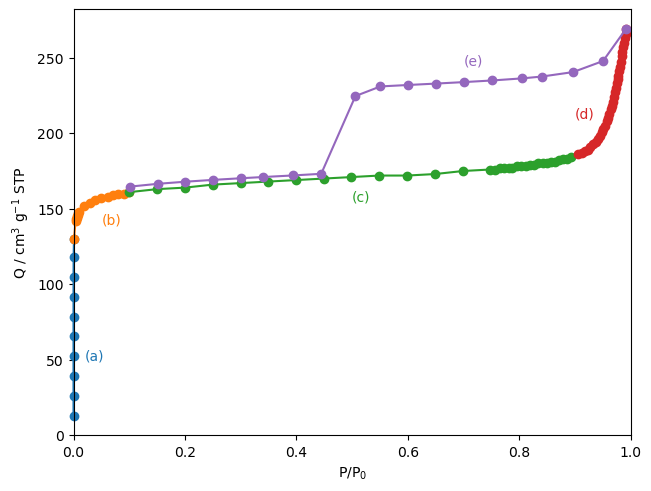
\includegraphics[width=\columnwidth, keepaspectratio]{1-introduction/figs/isotherm_anatomy.png}
    \caption{An isotherm of \ce{N2} on a turbostratic carbon. The isotherm possesses (a) high uptake in the micropore region, indicating microporosity; (b) a sharp knee due to a narrow \acrshort{psd}; (c) a plateau in the medium pressure region due to formation of a monolayer this remains flat in the middle of the isotherm due to lack of mesoporosity; (d) high uptake as relative pressure approaches 1 showing external surface adsorption; and (e) a hysteresis loop due to capillary condensation.}
    \label{fig:isotherm_anatomy}
\end{figure}

The various adsorption behaviours of a porous material discussed in the previous section result in distinct and interpretable forms of the resultant isotherms. As a general rule, the relative amount of gas adsorpted in different pressure ranges gives an indication of the amount of porosity in the internal \gls{micropore} and \gls{mesopore} regions as well as the amount of external surface area. To demonstrate, a labelled isotherm is shown in figure \ref{fig:isotherm_anatomy}. High adsorption in the low pressure region indicates the presence of \glspl{micropore}, while an increase in uptake at pressures around the midpoint of the isotherm indicate mesoporosity. If there is a plateau in the middle of the isotherm, this typically indicates that a monolayer has formed. The curvature of the isotherm prior to the plateau (the adsorption `knee') is indicative of the breadth of the \acrshort{psd}; a gentle knee shows a broad \acrshort{psd}, while a sharp knee indicates that pore sizes are narrowly distributed. Finally, high uptake as relative pressure approaches 1 are indicative of adsorption on the external surface, showing that the material is non-porous or macroporous.\citep{Thommes2015Physisorption} \acrshort{iupac} has designated eight distinct isotherm types.\citep{Thommes2015Physisorption, Sing1985} These need not be discussed in full detail here - it is sufficient to state that types I(a) and (b) isotherms are indicative of microporosity, while IV(a), IV(b) and V are seen on isotherms with high mesoporosity. Nonporous samples typically exhibit type II, III or VI isotherms. The variation in shapes can be indicative of surface chemistry and/or pore size hierarchy.\citep{thommes2014physical, monson2012understanding} Of course as a lot of materials exhibit multiple types of porosity, many materials exhibit characteristics of multiple isotherm types.\citep{Thommes2015Physisorption} 

Apart from the general isotherm types, the presence of hysteresis - i.e. desorption releasing less \gls{adsorbate} than is taken up during adsorption at an identical relative pressure - is indicative of capillary condensation (see section \ref{ss:pore_filling}.\citep{thommes2014physical, monson2012understanding, landers2013density} As with characteristic isotherm types, \acrshort{iupac} has defined six distinct forms of hysteresis loop. Depending on the type of hyteresis loop, its presence may indicate adsorption metastability in an `open' pore, pore network effects and/or other forms of pore blocking.\citep{Thommes2015Physisorption} Each of the six hysteresis loops are associated with specific kinds of materials - for example H4 loops are frequently found in micro-mesoporous carbons, whereas H1 is typically associated with materials possessing uniform open mesopores.\citep{Thommes2015Physisorption, monson2012understanding}  

\newpage
\setcounter{opagenum}{\thepage}
\section[Publication I]{Publication I: Modulating the porosity of carbons for improved adsorption of hydrogen, carbon dioxide, and methane: a review}

\textbf{Contribution of the author}: The author designed and performed the literature review and wrote the manuscript.

\clearpage
%\BackupCounterGroup[backup-id=pub1]{pagebackup}
\newpage

\setlength{\originalVOffset}{\voffset}   
\setlength{\originalHOffset}{\hoffset}

\setlength{\voffset}{0cm}
\setlength{\hoffset}{0cm}
% too big for overleaf, try compilation later.
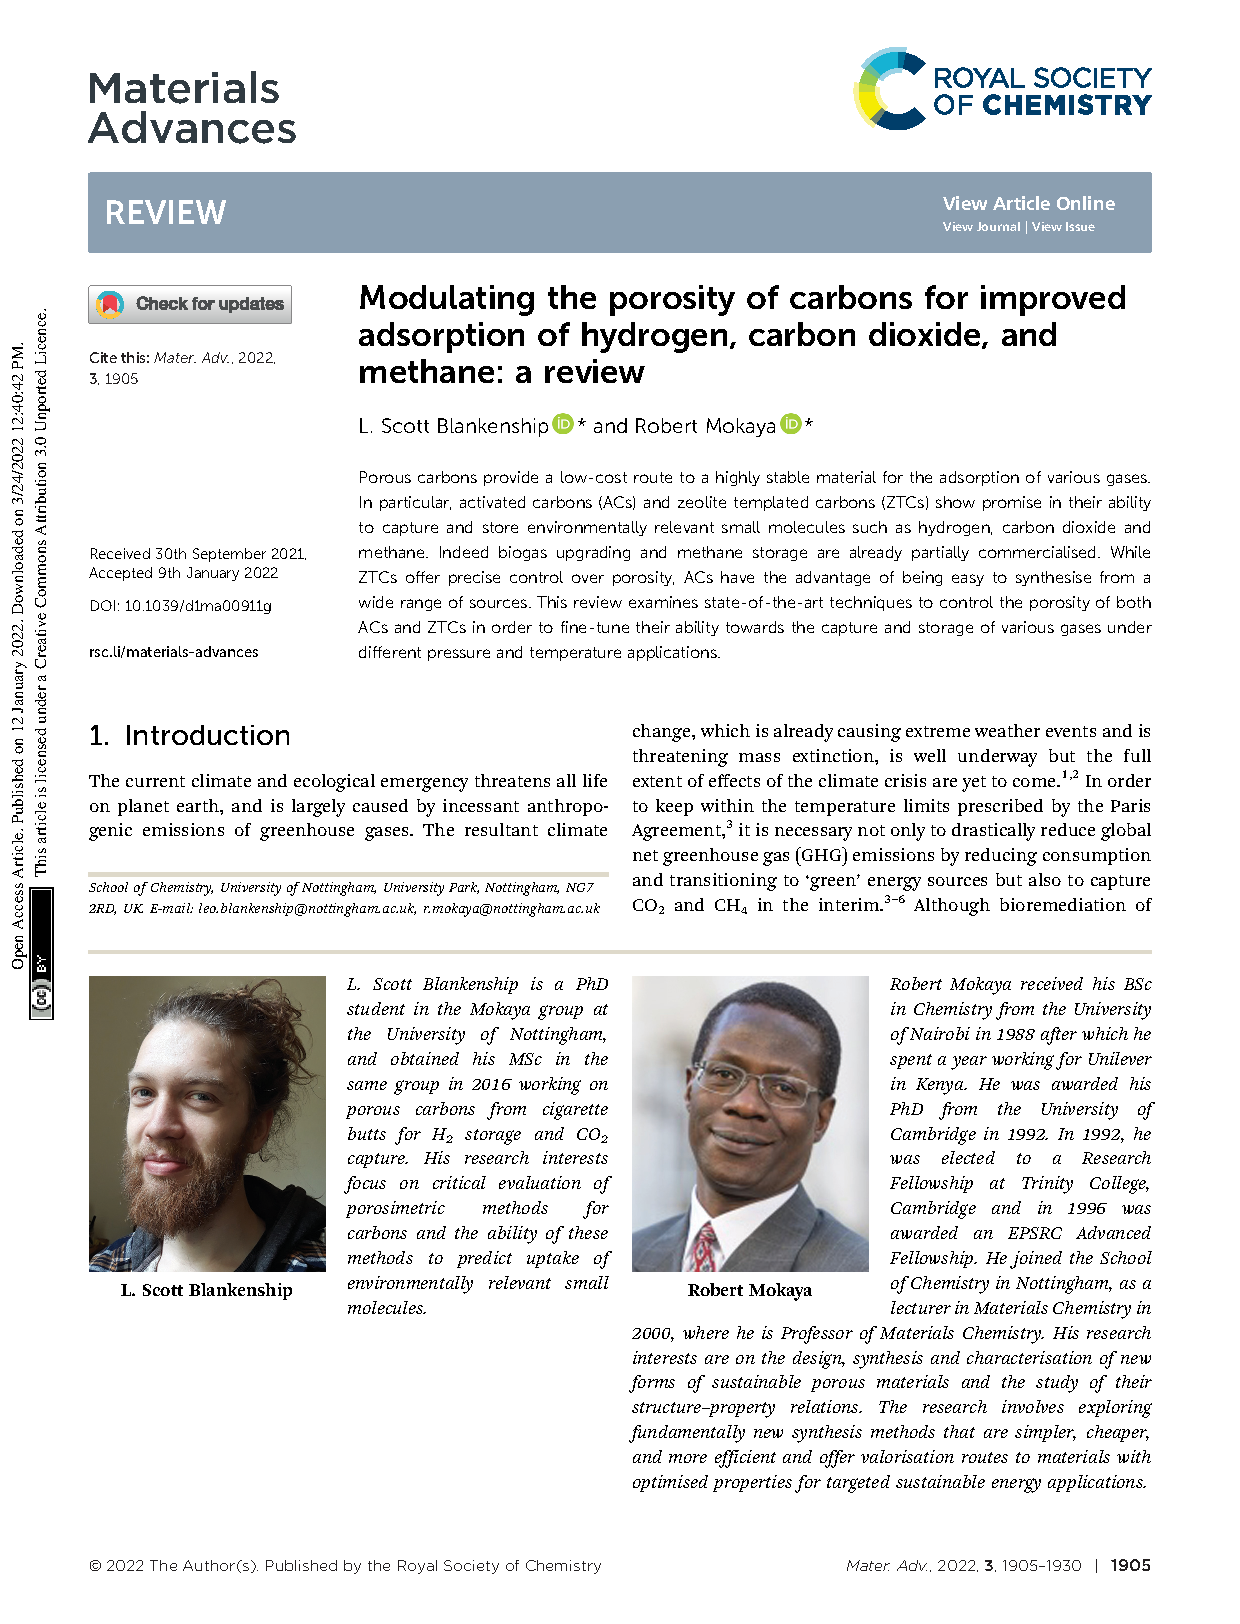
\includepdf[
    pagecommand={
    \setcounter{page}{\theopagenum}
    \thispagestyle{empty}
    },
    pages=-]{1-introduction/publication_01.pdf}
\setlength{\voffset}{\originalVOffset}
\setlength{\hoffset}{\originalHOffset}

\clearpage
%\RestoreBackupCounterGroup[backup-id=pub1]{pagebackup}

\bibliographystyle{rsc}
\bibliography{bibliography/bib}